% Provenance (never printed): the distribution strand of ../economics_series.md (grade 9: mean and median income; shares
% by fifths; inequality inside and between countries; the world distribution over time; world poverty fell while
% inequality rose inside some countries). Brief: sources/book1/BRIEFS.md, g9-07. A description chapter: no model box.
% Lorenz curve and Gini are grade 11's. The world distribution is built from PIP survey percentiles (nearest survey
% within 3 years of 1990 and 2019, weighted by population): the method is in the figdata docstring and the measure box.
% Chart data: figdata/grade-9/07-income-distribution. Ledger: g9:pip-welfare-aggregate.
\chapter{Who Earns What: Income Distribution}\label{ch:g9:income-distribution}

\begin{openingchart}{The world's people by income or consumption per person per day, around 1990 and around
2019, in dollars of 2021 at purchasing-power parity (times-ten scale): millions of people in each band. Each
country's household survey nearest the year (within three years) is used; the 1990 curve covers
$84\,\%$ of the world's population (85 countries), the 2019 curve $98\,\%$ (144 countries). The dashed line is
the international poverty line of 3 dollars a day.}{World \omterm{def:g8:banks-saving-interest:bank}{Bank}, Poverty and Inequality Platform (survey
percentiles) and World Development Indicators (SP.POP.TOTL)}
\begin{tikzpicture}
\begin{axis}[omrecord, xmin=-1, xmax=2.6, ymin=0, ymax=850, width=0.9\linewidth, height=0.45\linewidth,
  xtick={-1,0,1,2}, xticklabels={0.1, 1, 10, 100}, xlabel={Dollars per person per day (times-ten scale)},
  ylabel={Millions of people}, legend pos=north east]
\addplot[omThm, thick, const plot mark mid] table[x=logmid, y=y1990]
  {figdata/grade-9/07-income-distribution/out/world_distribution.csv};
\addplot[omDef, thick, const plot mark mid] table[x=logmid, y=y2019]
  {figdata/grade-9/07-income-distribution/out/world_distribution.csv};
\draw[black!60, dashed] (axis cs:0.477,0) -- (axis cs:0.477,850);
\legend{around 1990, around 2019}
\end{axis}
\end{tikzpicture}
\end{openingchart}

% figdata: facts peak_1990 2.82, peak_2019 5.62; below_line_1990 45.3, below_line_2019 9.5
Around 1990, the largest group of the world's people lived on about 3 dollars a day, and $45\,\%$ of the
people covered lived on less than 3 dollars a day. Around 2019, the largest group lived on about 6 dollars
a day, and fewer than $10\,\%$ were below the line. The world's population grew, and the whole hump moved
to the right.

\begin{recall}
The mean of a list of numbers is their sum divided by how many there are; the median is the middle value
once they are sorted. The \omterm{def:g6:poverty:poverty-rate}{poverty rate} is the share of people below a \omterm{def:g6:poverty:poverty-line}{poverty line}; the international line
is 3 dollars a day per person (\cref{ch:g6:poverty}). Amounts in different countries are compared with
purchasing-power conversion (\cref{ch:g9:exchange-rates-and-purchasing-power}).
\end{recall}

\section{Mean and median income}

\begin{definition}[Income distribution]\label{def:g9:income-distribution:income-distribution}
The \emph{income distribution}\index{income distribution} of a group of people or \omterm{def:g7:households:household}{households} is the list
of their \omterm{def:g7:households:income}{incomes}: how many have each level of \omterm{def:g7:households:income}{income}.
\end{definition}

\begin{definition}[Mean income]\label{def:g9:income-distribution:mean-income}
The \emph{mean income}\index{mean income} of a group is its total \omterm{def:g7:households:income}{income} divided by the number of people
(or \omterm{def:g7:households:household}{households}) in it.
\end{definition}

\begin{definition}[Median income]\label{def:g9:income-distribution:median-income}
The \emph{median income}\index{median income} of a group is the \omterm{def:g7:households:income}{income} of the person (or \omterm{def:g7:households:household}{household}) in the
middle when everyone is ranked from the lowest \omterm{def:g7:households:income}{income} to the highest: half have less, half have more.
\end{definition}

\begin{omfigure}
\begin{tikzpicture}[x=0.095cm, y=1cm, font=\scriptsize]
  \draw[->] (0,0) -- (128,0);
  \node[below=12pt] at (64,0) {thousand dalens a year};
  \foreach \v in {0,20,...,120} \draw (\v,0.08) -- (\v,-0.08) node[below] {\v};
  \foreach \v in {12,14,15,17,18,20,22,25,120} \fill[omDef] (\v,0.3) circle (2.2pt);
  \draw[omThm, thick] (18,0.05) -- (18,0.95) node[above] {median 18};
  \draw[black, thick, dashed] (29.2,0.05) -- (29.2,0.95) node[above right=-2pt] {mean 29.2};
\end{tikzpicture}

{\small Nine invented \omterm{def:g7:households:household}{households}. One high \omterm{def:g7:households:income}{income} pulls the mean far above the median, which most
\omterm{def:g7:households:household}{households} are close to.}
\end{omfigure}

When a few \omterm{def:g7:households:income}{incomes} are very high, the mean is pulled above the median. In the nine \omterm{def:g7:households:household}{households} above, the
total is 263 thousand dalens and the mean $263 \div 9 = 29.2$; the median, the fifth \omterm{def:g7:households:income}{income}, is 18. Eight of
the nine \omterm{def:g7:households:household}{households} have less than the mean. \omterm{def:g9:income-distribution:income-distribution}{Income distributions} usually look like this, so the median
often says more about a typical \omterm{def:g7:households:household}{household}.

\section{Shares by fifths}

\begin{definition}[Income share of a fifth]\label{def:g9:income-distribution:fifth-share}
Rank the people (or \omterm{def:g7:households:household}{households}) of a country from the lowest \omterm{def:g7:households:income}{income} to the highest and cut the list into
five groups of equal size, the fifths. The \emph{income share of a fifth}\index{income share of a fifth}
is that group's \omterm{def:g7:households:income}{income} as a percentage of the total \omterm{def:g7:households:income}{income} of all.
\end{definition}

\begin{omfigure}
\begin{tikzpicture}
\begin{axis}[omrecord, ybar, bar width=18pt, ymin=0, ymax=55, height=0.36\linewidth, width=0.6\linewidth,
  xmin=0.5, xmax=5.5,
  xtick={1,...,5}, xticklabels={poorest, second, middle, fourth, richest}, xticklabel style={font=\footnotesize},
  ylabel={Share of income (percent)}, nodes near coords, nodes near coords style={font=\scriptsize}]
\addplot[fill=omDef, draw=none] table[x=fifth, y=income] {figdata/grade-9/07-income-distribution/out/town.csv};
\draw[black!60, dashed] (axis cs:0.5,20) -- (axis cs:5.5,20) node[pos=0.06, above, font=\scriptsize] {20};
\end{axis}
\end{tikzpicture}

{\small Shares by fifths in an invented town. If everyone had the same \omterm{def:g7:households:income}{income}, every bar would reach the
dashed line at $20\,\%$.}
\end{omfigure}

In the invented town, the richest fifth receives $47\,\%$ of all \omterm{def:g7:households:income}{income} and the poorest fifth $6\,\%$: the
richest fifth's share is nearly eight times the poorest fifth's.

\begin{measure}[Income or consumption]
% ledger: g9:pip-welfare-aggregate
\omterm{def:g7:households:household}{Household} surveys ask either about \omterm{def:g7:households:income}{income} or about consumption, the value of what the \omterm{def:g7:households:household}{household} buys and
uses. Each country chooses the one it can measure more accurately. \omterm{def:g7:households:income}{Income} is hard to measure where many
people work for themselves or without a contract, or grow their own food, which is often the case in poorer
countries; there, surveys usually measure consumption (Poverty and Inequality Platform handbook). \omterm{def:g7:households:household}{Households}
smooth their consumption over time, so shares measured on consumption and on \omterm{def:g7:households:income}{income} are not the same
thing: two countries' numbers are best compared when they measure the same one.
\end{measure}

\section{Inequality inside a country}

\begin{definition}[Inequality within a country]\label{def:g9:income-distribution:within}
\emph{Inequality within a country}\index{inequality within a country} is how far the \omterm{def:g7:households:income}{incomes} of its people
differ from one another, measured for example by the \omterm{def:g7:households:income}{income} share of the richest fifth.
\end{definition}

% figdata: top_fifth_share; facts top_* first and last
\begin{omchart}{Share of income or consumption received by the richest fifth, percent, in survey years since
1980. Brazil, the United Kingdom, Sweden and the United States measure income; China and India measure
consumption in most years.}{World \omterm{def:g8:banks-saving-interest:bank}{Bank}, World Development Indicators (SI.DST.05TH.20)}
\begin{tikzpicture}
\begin{axis}[omrecord, width=0.9\linewidth, height=0.45\linewidth, xmin=1980, xmax=2024, ymin=25, ymax=70,
  xtick={1980,1990,2000,2010,2020}, xticklabel style={/pgf/number format/1000 sep={}}, xlabel={Year},
  ylabel={Richest fifth's share (percent)}, unbounded coords=jump, mark size=1pt, legend columns=3,
  legend style={at={(0.5,1.03)}, anchor=south, font=\footnotesize}]
\addplot[black!70, thick, mark=*] table[x=year, y=BRA] {figdata/grade-9/07-income-distribution/out/top_fifth_share.csv};
\addplot[omDef, thick, mark=*] table[x=year, y=USA] {figdata/grade-9/07-income-distribution/out/top_fifth_share.csv};
\addplot[omThm, thick, mark=*] table[x=year, y=CHN] {figdata/grade-9/07-income-distribution/out/top_fifth_share.csv};
\addplot[omThm!50, thick, dashed, mark=*] table[x=year, y=IND] {figdata/grade-9/07-income-distribution/out/top_fifth_share.csv};
\addplot[omDef!50, thick, dashed, mark=*] table[x=year, y=GBR] {figdata/grade-9/07-income-distribution/out/top_fifth_share.csv};
\addplot[black!40, thick, dotted, mark=*] table[x=year, y=SWE] {figdata/grade-9/07-income-distribution/out/top_fifth_share.csv};
\legend{Brazil, United States, China, India, United Kingdom, Sweden}
\end{axis}
\end{tikzpicture}
\end{omchart}

The richest fifth's share was 62 percent in Brazil in 1981 and 55 in 2024; in the United States it rose from
41 percent in 1980 to 47 in 2024; in China from 37 in 1981 to 44 in 2022. In Sweden it was 33 in 1981 and 37
in 2023. Inequality inside a country can rise or fall, and it has done both.

\begin{omfigure}
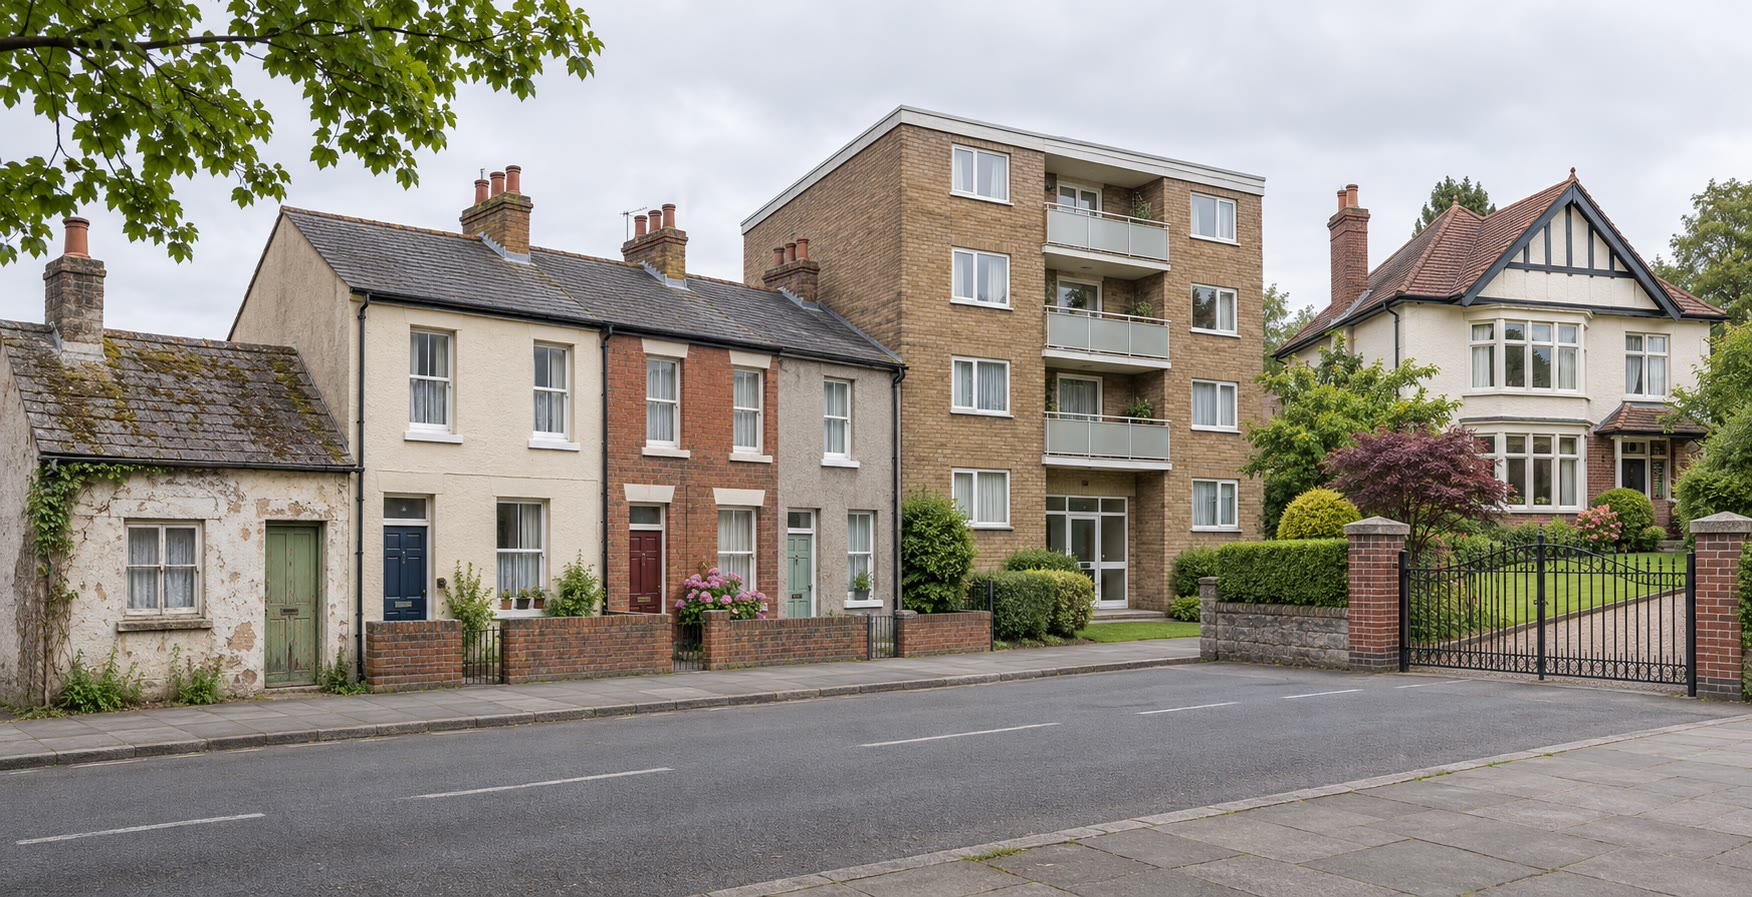
\includegraphics[width=0.5\linewidth]{images/book1/ai/g9-distribution-street-of-houses.jpg}

{\small One street, many \omterm{def:g7:households:income}{incomes}: homes of very different sizes side by side.}
\end{omfigure}

\section{Between countries}

\begin{definition}[Inequality between countries]\label{def:g9:income-distribution:between}
\emph{Inequality between countries}\index{inequality between countries} is how far the \omterm{def:g9:income-distribution:mean-income}{mean incomes} of
countries differ from one another.
\end{definition}

A person's \omterm{def:g7:households:income}{income} depends a great deal on the country where they live. \omterm{def:g8:gdp:gdp-per-person}{GDP per person}, at
purchasing-power parity, is about 8 times higher in the United States than in India
(\cref{ch:g9:exchange-rates-and-purchasing-power}): a \omterm{def:g7:households:household}{household} in the middle of India's distribution and one
in the middle of the United States' distribution are far apart because their countries are.

\section{The world distribution, then and now}

\begin{definition}[World income distribution]\label{def:g9:income-distribution:world-distribution}
The \emph{world income distribution}\index{world income distribution} is the \omterm{def:g9:income-distribution:income-distribution}{income distribution} of all the
world's people taken together, as if they lived in one country, after purchasing-power conversion.
\end{definition}

\begin{measure}[World distribution]
The opening chart is built from each country's \omterm{def:g7:households:household}{household} survey, cut into a hundred groups of equal size
from the poorest to the richest, each with its \omterm{def:g9:income-distribution:mean-income}{mean income} or consumption in dollars of 2021 at
purchasing-power parity. For each country, the survey nearest to 1990 (or 2019), within three years, is
used, and each hundredth stands for one hundredth of the country's population in that year. All the groups
of all the countries are then sorted into bands of \omterm{def:g7:households:income}{income}, and the people in each band are added up.
Countries without a survey near the year are left out: in 1990 they hold $16\,\%$ of the world's people.
\end{measure}

% figdata: facts median_1990 3.33, median_2019 8.8; chn_median 1.71 -> 12.02 (surveys 1990, 2019); ind_median
% 3.09 -> 5.51 (surveys 1993, 2022); chn_ind_share_of_below_1990 66.8
The world's median moved from about 3.3 dollars a day around 1990 to about 8.8 around 2019. Much of the
change comes from the two most populous countries. In China's surveys, the median went from 1.7 dollars a day
in 1990 to 12.0 in 2019; in India's, from 3.1 in 1993 to 5.5 in 2022.

\section{Two facts together}

Two facts hold at once. The share of the world's people below 3 dollars a day fell from about $45\,\%$ to
under $10\,\%$ between 1990 and 2019. And inside some countries, such as the United States and China, the
richest fifth's share rose. They do not contradict each other. Around 1990, two thirds of the people below the line
in the opening chart lived in China and India, whose \omterm{def:g9:income-distribution:mean-income}{mean incomes} then grew fast; and a country's poorest can become richer even while the richest
fifth's share rises, when the whole country's \omterm{def:g7:households:income}{income} grows fast enough.

\section{Exercises}

\begin{exercise}[$\star$]\label{exo:g9:income-distribution:1}
Use the opening chart. At about what \omterm{def:g7:households:income}{income} per day is each curve highest, around 1990 and around 2019?
\end{exercise}

\begin{exercise}[$\star$]\label{exo:g9:income-distribution:2}
Nine \omterm{def:g7:households:household}{households} have \omterm{def:g7:households:income}{incomes} of 8, 9, 10, 10, 11, 12, 13, 15 and 40 thousand dalens a year. Compute the mean
and the median.
\end{exercise}

\begin{exercise}[$\star$]\label{exo:g9:income-distribution:3}
In an invented town, the five fifths receive 30, 50, 70, 100 and 250 thousand dalens in total. Compute each
fifth's share of total \omterm{def:g7:households:income}{income}.
\end{exercise}

\begin{exercise}[$\star$]\label{exo:g9:income-distribution:4}
Use the top-fifth chart. What was the richest fifth's share in Sweden in 2023 and in Brazil in 2024?
\end{exercise}

\begin{exercise}[$\star\star$]\label{exo:g9:income-distribution:5}
Brenland's 2,000 surveyed \omterm{def:g7:households:household}{households} have a total \omterm{def:g7:households:disposable-income}{disposable income} of $49.84$ million dalens, and the
poorest fifth receives $11.1\,\%$ of it. Compute the mean \omterm{def:g7:households:disposable-income}{disposable income} of all \omterm{def:g7:households:household}{households} and of the
\omterm{def:g7:households:household}{households} in the poorest fifth.
\end{exercise}

\begin{exercise}[$\star\star$]\label{exo:g9:income-distribution:6}
A tenth \omterm{def:g7:households:household}{household}, with an \omterm{def:g7:households:income}{income} of 200 thousand dalens, joins the nine \omterm{def:g7:households:household}{households} of exercise 2. Compute
the new mean and median. Which one changed more?
\end{exercise}

\begin{exercise}[$\star\star$]\label{exo:g9:income-distribution:7}
China's richest fifth received $37.2\,\%$ in 1981 and $43.7\,\%$ in 2022. By how many percentage points did
the share change?
\end{exercise}

\begin{exercise}[$\star\star$]\label{exo:g9:income-distribution:8}
In two invented countries, the \omterm{def:g9:income-distribution:mean-income}{mean income} is 60 dollars a day in the first and 6 in the second. The
second's \omterm{def:g9:income-distribution:mean-income}{mean income} doubles; the first's rises by $20\,\%$. How many times the second's mean is the first's,
before and after?
\end{exercise}

\begin{exercise}[$\star\star$]\label{exo:g9:income-distribution:9}
What observation would contradict the statement ``the share of the world's people below 3 dollars a day fell
between 1990 and 2019''? Could the way the opening chart was built hide such an observation?
\end{exercise}

\begin{exercise}[$\star\star\star$]\label{exo:g9:income-distribution:10}
In the invented town of the shares chart (6, 10, 15, 22, 47 percent), \omterm{def:g8:taxes-and-public-spending:tax}{taxes} take an amount equal to $5\,\%$ of
total \omterm{def:g7:households:income}{income} from the richest fifth and give it to the poorest fifth. Compute the new shares.
\end{exercise}

\begin{exercise}[$\star\star\star$]\label{exo:g9:income-distribution:11}
Put in one table: the share of the world's people below 3 dollars a day around 1990 and 2019, and the richest
fifth's share in the United States (1980, 2024) and China (1981, 2022). Explain how both trends can be true.
\end{exercise}

\begin{exercise}[$\star\star\star$]\label{exo:g9:income-distribution:12}
A country's fifths' shares are the same in 2000 and in 2020. Does this mean that the same \omterm{def:g7:households:household}{households} were
in the poorest fifth in both years? What would you need to know?
\end{exercise}

\section{Problem: Brenland's Fifths}

\begin{problem}[{Weekend problem --- mean and median of Brenland's household incomes, shares by fifths before
and after taxes and transfers, and the poverty line in dalens}]
\label{pb:g9:income-distribution:1}
Brenland is invented. Its 2025 survey of 2,000 \omterm{def:g7:households:household}{households} gives each \omterm{def:g7:households:household}{household}'s gross \omterm{def:g7:households:income}{income} (before \omterm{def:g8:taxes-and-public-spending:tax}{taxes}
and \omterm{def:g7:households:transfer}{transfers}) and \omterm{def:g7:households:disposable-income}{disposable income} (after them). Shares are of total \omterm{def:g7:households:household}{household} \omterm{def:g7:households:income}{income}, with \omterm{def:g7:households:household}{households}
ranked by that \omterm{def:g7:households:income}{income}.

\begin{center}\small
\begin{tabular}{lrrrrr}
\toprule
Fifth & poorest & second & middle & fourth & richest \\
\midrule
Gross \omterm{def:g7:households:income}{income} (percent) & 8.1 & 14.0 & 17.5 & 23.0 & 37.4 \\
\omterm{def:g7:households:disposable-income}{Disposable income} (percent) & 11.1 & 15.0 & 17.9 & 22.5 & 33.5 \\
\bottomrule
\end{tabular}
\end{center}

\medskip
\noindent\textbf{Part I --- Mean and median.}
\begin{enumerate}
  \item The total \omterm{def:g7:households:disposable-income}{disposable income} of the 2,000 \omterm{def:g7:households:household}{households} is $49.84$ million dalens. Compute the mean.
  \item The median \omterm{def:g7:households:disposable-income}{disposable income} is 22,265 dalens. Is it above or below the mean?
  \item Explain why.
\end{enumerate}

\medskip
\noindent\textbf{Part II --- Before and after taxes and transfers.}
\begin{enumerate}[resume]
  \item How many times the poorest fifth's share is the richest fifth's share of gross \omterm{def:g7:households:income}{income}?
  \item The same for \omterm{def:g7:households:disposable-income}{disposable income}.
  \item Which fifths have a larger share after \omterm{def:g8:taxes-and-public-spending:tax}{taxes} and \omterm{def:g7:households:transfer}{transfers}, and which a smaller one?
  \item Mean gross \omterm{def:g7:households:income}{income} is 26,818 dalens, mean \omterm{def:g8:taxes-and-public-spending:tax}{tax} 3,391 and mean \omterm{def:g7:households:transfer}{transfers} 1,493. Check that mean
        \omterm{def:g7:households:disposable-income}{disposable income} is the answer to question 1.
\end{enumerate}

\medskip
\noindent\textbf{Part III --- The poverty line in dalens.} Suppose that a dollar of purchasing power buys as
much in Brenland as 2 dalens.
\begin{enumerate}[resume]
  \item What is the line of 3 dollars a day per person in dalens a day?
  \item In dalens a year (365 days)?
  \item For a \omterm{def:g7:households:household}{household} of two people?
  \item The poorest fifth's \omterm{def:g7:households:household}{households} have a mean \omterm{def:g7:households:disposable-income}{disposable income} of 13,869 dalens. How many times the
        line for two people is that?
  \item Can you tell from these numbers whether any \omterm{def:g7:households:household}{household} in Brenland is below the line? What would you
        need?
  \item By how many percentage points do \omterm{def:g8:taxes-and-public-spending:tax}{taxes} and \omterm{def:g7:households:transfer}{transfers} lower the richest fifth's share?
\end{enumerate}
\end{problem}
